%
%PEN INSTRUCTION
%
\documentclass[10pt,a4j]{jarticle}
%\pagestyle{empty}
\usepackage{amsmath}
\usepackage{amssymb}
\usepackage{epsfig}
\usepackage{color}
%\usepackage{txfonts}

%\setlength{\topmargin}{-0mm}
%\setlength{\oddsidemargin}{-0mm}
%\setlength{\textheight}{252mm}
%\setlength{\textwidth}{180mm}

%---------- 箇条書き -----------

\newenvironment{itemize2}%  
{%
   \begin{list}{$\bullet$\ \ }% 見出し記号/直後の空白を調節
   {%
      \setlength{\itemindent}{0pt}
      \setlength{\leftmargin}{3zw}%  左のインデント
      \setlength{\rightmargin}{0zw}% 右のインデント
      \setlength{\labelsep}{0zw}%    黒丸と説明文の間
      \setlength{\labelwidth}{3zw}%  ラベルの幅
      \setlength{\itemsep}{0em}%     項目ごとの改行幅
      \setlength{\parsep}{0em}%      段落での改行幅
      \setlength{\listparindent}{0zw}% 段落での一字下り
   }
}{%
   \end{list}%
}
%---------- 番号つき箇条書き -----------

\newcounter{enum2}
\newenvironment{enumerate2}{%
   \begin{list}%
   {%
      \arabic{enum2}.\ \,%  見出し記号/直後の空白を調節
   }%
   {%
      \usecounter{enum2}
      \setlength{\itemindent}{0zw}%  ここは 0 に固定
      \setlength{\leftmargin}{3zw}%  左のインデント
      \setlength{\rightmargin}{0zw}% 右のインデント
      \setlength{\labelsep}{0zw}%    黒丸と説明文の間
      \setlength{\labelwidth}{3zw}%  ラベルの幅
      \setlength{\itemsep}{0em}%     項目ごとの改行幅
      \setlength{\parsep}{0em}%      段落での改行幅
      \setlength{\listparindent}{0zw}% 段落での一字下り
   }
}{%
   \end{list}%
}
\setlength{\topsep}{0pt}
\setlength{\itemsep}{10pt}
\setlength{\parsep}{0mm}
\setlength{\itemindent}{50mm}

\labelsep 20mm
\labelwidth 50mm
\leftmargin 100mm
\newcommand{\ExerciseTitle}[1]{%
  \begin{center}\Large
    \textbf{PEN マニュアル Q \& A} \qquad \texttt{#1}
  \end{center}%
}


\renewcommand{\baselinestretch}{1.0}

\begin{document}

\noindent
\begin{flushright}
{\small	2009/02/16}
\end{flushright}
\begin{center}
\begin{LARGE}
{\bf{PENの動作を制御する}}
\end{LARGE}
\end{center}

Property.ini 内で指定できる設定項目は以下の通り。
パラメータは起動時に読み込まれる。

\section{変数宣言の要/不要の設定}

変数宣言の要/不要を設定する。

\begin{quotation}

\noindent [使用例]\\
~~~~{\bf{executer.var.declaration=0}}\\
\ \\ 
設定値は以下の通り(デフォルト値は0)。\\

\begin{tabular}{c|l||cl}
\hline
\multicolumn{2}{c||}{設定値} & \multicolumn{2}{c}{変数宣言がない場合の出力}\\
\hline
0 & 変数宣言必須 &  & エラー \\
\hline
1 & 変数宣言不要 &  & 警告表示 \\
\hline
2 & 変数宣言不要 &  & エラーと警告表示なし \\
\hline
\end{tabular}

\end{quotation}

\section{配列の添字の範囲を設定}
配列を宣言して変数を確保するとき、添字の範囲を決めることができる。

\begin{quotation}
\noindent [使用例]\\
~~~~{\bf{executer.array.origin=0}}\\
\ \\ 
設定値は以下の通り。\\

\begin{tabular}{c|l}
\hline
設定値  & 配列 X[n] を宣言した場合 \\
\hline
0       & X[0],...,X[n]  の要素を確保する (デフォルト値) \\
\hline
1       & X[0],...,X[n-1]の要素を確保する \\
\hline
2       & X[1],...,X[n]  の要素を確保する \\
\hline
\end{tabular}

%\begin{tabular}{ccl}
%設定値 & : & 配列 X[n] を宣言した場合 \\
%0      & : & X[0],...,X[n]  の要素を確保する (デフォルト値) \\
%1      & : & X[0],...,X[n-1]の要素を確保する \\
%2      & : & X[1],...,X[n]  の要素を確保する \\
%\end{tabular}

\end{quotation}

\section{描画ウィンドウの原点の設定}

描画ウィンドウで座標を指定するときの原点を設定する。

\begin{quotation}
\noindent [使用例]\\
~~~~{\bf{executer.graphic.origin=0}}\\
\ \\
設定値は以下の通り。\\

\begin{tabular}{c|l}
\hline
0 & 左上を原点にする (デフォルト値) \\
\hline
1 & 左下を原点にする \\
\hline
\end{tabular}
\end{quotation}

%\begin{tabular}{ccl}
%0 & : & 左上を原点にする (デフォルト値) \\
%1 & : & 左下を原点にする \\
%\end{tabular}
%\end{quotation}

\section{入力支援ボタンの定義を別ファイルで行う}

入力支援ボタンの設定を別ファイルに記述しておくことができる。
定義ファイルまでのパスを設定値に記述しておくと、
PENはその定義ファイルを用いて起動する。

通常は、このファイルを指定せずにPENを起動することができる。

\begin{quotation}
\noindent [使用例]\\
~~~~{\bf{ pen.button.path=./ButtonList.ini}}

\end{quotation}

\section{フォントサイズを大きくして起動する設定}

起動時のフォントサイズを大きくすることができる。

\begin{quotation}
\noindent [使用例]\\
~~~~{\bf{pen.teacher.flag=0}}\\
\ \\
設定値は以下の通り。\\

\begin{tabular}{c|l}
\hline
0 & 通常の大きさ (デフォルト値)\\
\hline
1 & フォントサイズを拡大して起動 \\
\hline
\end{tabular}\\

%\begin{tabular}{ccl}
%0 & : & 通常起動 \\
%1 & : & フォントサイズを大きくして起動 \\
%\end{tabular}

図~\ref{fig:font01}は拡大したサイズ、図~\ref{fig:font02}は標準サイズでの表示。

\end{quotation}

\begin{figure}[!h]
\begin{minipage}{50zw}
\begin{center}
\epsfig{file=./eps/pen_font_large.ps, width=5.5in}
\caption{$\!\!\!\!$\colorbox{white}{{\textcolor{white}{:}}}拡大サイズ }
\label{fig:font01}
\end{center}
\end{minipage}
\ \\
\ \\
\begin{minipage}{50zw}
\begin{center}
\epsfig{file=./eps/pen_font_small.ps, width=5.5in}
\caption{$\!\!\!\!$\colorbox{white}{{\textcolor{white}{:}}}標準サイズ}
\label{fig:font02}
\end{center}
\end{minipage}

\end{figure}


\section{デバックモードでの起動}
デバッグモードを利用することができる。
デバッグ結果(構文解析されたツリー)はコンソールに出力される。

\begin{quotation}
\noindent [使用例] デバッグモードでの起動方法\\
~~~~{\bf{pen.debug.flag=1}}\\
~~~~と設定し、コマンドプロンプト上で、
~~~~> java -jar PEN.jar
~~~~と入力し起動する。

\ \\
設定値は以下の通り。\\

\begin{tabular}{c|l}
\hline
0 & 通常起動 (デフォルト値) \\
\hline
1 & debugモードで起動 \\
\hline
\end{tabular}

%\begin{tabular}{ccl}
%0 & : & 通常起動 (デフォルト値) \\
%1 & : & debugモードで起動 \\
%\end{tabular}

\end{quotation}

\section{エラー時のダンプ動作設定}
xDNCLの実行時にエラーが発生した場合、
dumpファイルを出力させるように設定することができる。
また、出力先の指定もできる。

\begin{quotation}
\noindent [使用例]\\
~~~~{\bf{pen.dump.flag=0}}\\
\ \\
設定値は以下の通り。\\

\begin{tabular}{c|l}
\hline
0 & dumpファイルを生成しない (デフォルト値) \\
\hline
1 & dumpファイルを生成する \\
\hline
\end{tabular}

%\begin{tabular}{ccl}
%0 & : & dumpファイルを生成しない (デフォルト値) \\
%1 & : & dumpファイルを生成する \\
%\end{tabular}

\end{quotation}

\subsection{dumpファイルの暫定保存先を指定}
dumpファイルの作成を指定した場合、ファイルの一時保存先を指定することができる。
\begin{quotation}
\begin{tabular}{l}
出力先を設定しなければ HOMEディレクトリへ出力される。\\
(Windowsの場合は、C:¥Document~and~Settings¥ ユーザー名) \\
\ \\
出力先の指定方法は、\\
{\bf{pen.dump.tempdir=一時保存先}} \\
\end{tabular}
\end{quotation}

\subsection{一時保存したdumpファイルの最終保存先を指定}
%# (ログファイル保存先にdumpファイルを移動)
dumpファイルの作成を指定した場合、ファイルの最終保存先を指定することができる。
\begin{quotation}

\begin{tabular}{l}
出力先を設定しなければ HOMEディレクトリへ出力される。\\
(Windowsの場合は、C:¥Document\ and\ Settings¥ユーザー名) \\
出力されるファイル名は、「ユーザー名-コンピュータ名-数字.log」となる。\\
\ \\
出力先の指定方法は、\\
{\bf{pen.dump.destdir=ログファイル保存先}} \\
\end{tabular}

\end{quotation}

\end{document}


